\documentclass{sigchi}

% Use this command to override the default ACM copyright statement (e.g. for preprints). 
% Consult the conference website for the camera-ready copyright statement.


%% EXAMPLE BEGIN -- HOW TO OVERRIDE THE DEFAULT COPYRIGHT STRIP -- (July 22, 2013 - Paul Baumann)
% \toappear{Permission to make digital or hard copies of all or part of this work for personal or classroom use is 	granted without fee provided that copies are not made or distributed for profit or commercial advantage and that copies bear this notice and the full citation on the first page. Copyrights for components of this work owned by others than ACM must be honored. Abstracting with credit is permitted. To copy otherwise, or republish, to post on servers or to redistribute to lists, requires prior specific permission and/or a fee. Request permissions from permissions@acm.org. \\
% {\emph{CHI'14}}, April 26--May 1, 2014, Toronto, Canada. \\
% Copyright \copyright~2014 ACM ISBN/14/04...\$15.00. \\
% DOI string from ACM form confirmation}
%% EXAMPLE END -- HOW TO OVERRIDE THE DEFAULT COPYRIGHT STRIP -- (July 22, 2013 - Paul Baumann)


% Arabic page numbers for submission. 
% Remove this line to eliminate page numbers for the camera ready copy
\pagenumbering{arabic}

% Load basic packages
\usepackage{balance}  % to better equalize the last page
\usepackage{graphics} % for EPS, load graphicx instead
\usepackage{times}    % comment if you want LaTeX's default font
\usepackage{url}      % llt: nicely formatted URLs
\usepackage{caption}

\usepackage[]{algorithm2e}
\let\proof\relax
\let\endproof\relax
\usepackage{amsthm}
\newtheorem{theorem}{Theorem}

% llt: Define a global style for URLs, rather that the default one
\makeatletter
\def\url@leostyle{%
  \@ifundefined{selectfont}{\def\UrlFont{\sf}}{\def\UrlFont{\small\bf\ttfamily}}}
\makeatother
\urlstyle{leo}


% To make various LaTeX processors do the right thing with page size.
\def\pprw{8.5in}
\def\pprh{11in}
\special{papersize=\pprw,\pprh}
\setlength{\paperwidth}{\pprw}
\setlength{\paperheight}{\pprh}
\setlength{\pdfpagewidth}{\pprw}
\setlength{\pdfpageheight}{\pprh}

% Make sure hyperref comes last of your loaded packages, 
% to give it a fighting chance of not being over-written, 
% since its job is to redefine many LaTeX commands.
\usepackage[pdftex]{hyperref}
\hypersetup{
pdftitle={SIGCHI Conference Proceedings Format},
pdfauthor={LaTeX},
pdfkeywords={SIGCHI, proceedings, archival format},
bookmarksnumbered,
pdfstartview={FitH},
colorlinks,
citecolor=black,
filecolor=black,
linkcolor=black,
urlcolor=black,
breaklinks=true,
}

% create a shortcut to typeset table headings
\newcommand\tabhead[1]{\small\textbf{#1}}


% End of preamble. Here it comes the document.
\begin{document}
\definecolor{tovi}{rgb}{.3,0.75,0.5}
\definecolor{ryan}{rgb}{.3,.1,.5}
\definecolor{gray}{rgb}{.3,.3,.3}

%use these commands while writing
\newcommand {\bjoern}[1]{{\color{red}\bf{BH: #1}\normalfont}}
\newcommand {\valkyrie}[1]{{\color{blue}\bf{VS: #1}\normalfont}}
\newcommand {\tovi}[1]{{\color{tovi}\bf{TG: #1}\normalfont}}
\newcommand {\ryan}[1]{{\color{ryan}\bf{RMS: #1}\normalfont}}

%comment out the above and uncomment these for final submit
%\newcommand {\bjoern}[1]{}
%\newcommand {\valkyrie}[1]{}
%\newcommand {\tovi}[1]{}

\newcommand {\bt}[1]{\textbf{#1} \normalfont}
\newcommand{\squishlist}{
 \begin{list}{$\bullet$}
  { \setlength{\itemsep}{0pt}
     \setlength{\parsep}{3pt}
     \setlength{\topsep}{3pt}
     \setlength{\partopsep}{0pt}
     \setlength{\leftmargin}{1.5em}
     \setlength{\labelwidth}{1em}
     \setlength{\labelsep}{0.5em} } }
\newcommand{\squishend}{
  \end{list}  }


\title{A Series of Tubes: Adding Interactivity to 3D Prints\\ with Pipes and Hollow Chambers}

%\numberofauthors{6}
%\author{
%  \alignauthor Valkyrie Savage $\dagger \star$ \\
%    \email{valkyrie@eecs.berkeley.edu}\\
%  \alignauthor Ryan Schmidt $\dagger$ \\
%    \email{ryan.schmidt@autodesk.com}\\
%  \alignauthor Tovi Grossman $\dagger$ \\
%    \email{tovi.grossman@autodesk.com}\\
%  \alignauthor George Fitzmaurice $\dagger$ \\
%    \email{george.fitzmaurice@autodesk.com}\\
%  \alignauthor Bj\"orn Hartmann $\star$ \\
%    \email{bjoern@eecs.berkeley.edu}\\ 
%  \alignauthor $\star$ UC Berkeley EECS \\
%	           $\dagger$ Autodesk Research \\
%}

\numberofauthors{1}
\author{
  \alignauthor anonymized for peer review \\
}

\teaser{
\centering
    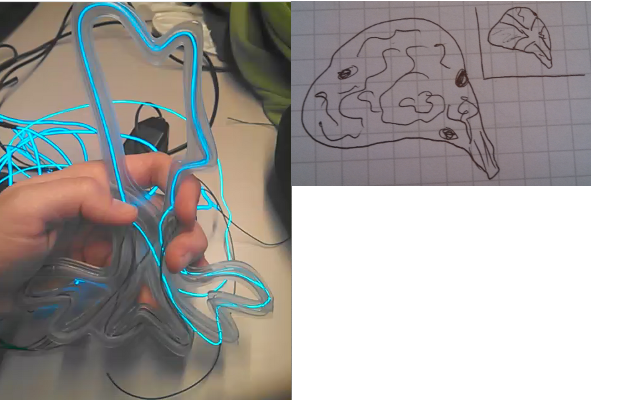
\includegraphics[width=\textwidth]{figures/placeholder/teaser.png}                                                                                                                                                                                                       
    \caption{A collection of interactive objects designed using our tool.  All have electronic sensing or actuation components which are routed through the \emph{interior} of the prints to preserve aesthetics.  In (a), objects manufactured on a hobbyist 3D printer.  In (b), those manufactured on industrial-grade printers.}
    \label{fig:teaser}
}

\maketitle

\begin{abstract}
3D printers offer extraordinary flexibilty in prototyping the shape and mechanical function of objects.  However, a 3D printer's role in prototyping interactive objects is still not clear.  We propose a general technique for adding interactivity by removing interior material to form pipes and cavities. These can be used to sense input and generate haptic as well as visible output. We describe the design space of pipes and hollow chambers for interaction design: a variety of openings, topologies, and inserted media for pipes create diverse inputs and outputs.  We present a technique and design tool for routing pipes of various topologies through the interior of 3D printed parts.  Our design tool is integrated into a 3D model manipulation program.  We use two distinct routing algorithms.  One, for creating particular points of interaction or integrating with existing electronics, allows users to select begin and end points for pipes, then uses A* path routing and physics-based simulation to minimize the bending energy of routed paths.  The second, for creating, e.g., novel neon signs, allows users to enter a description of paths to follow: for this we developed a novel routing algorithm and offer proof of key traits.  We present several totally tubular prototypes we created using this tool to show its flexibility and potential, as well as to explore new points in the pipe design space.
\end{abstract}

\keywords{
 Fabrication; 3D Printing; Interactive Objects; Design Tools
	%Prototyping; Electronics; Hardware \valkyrie{aw, let's keep it on one line. but what do we drop?} \bjoern{I emphasized the software contribution}
}


\classification{H.5.2 [User Interfaces (D.2.2, H.1.2, I.3.6)]:
Prototyping.} 

\input{Introduction}

\input{RelatedWork}

\input{DesignSpace}

\input{Tubes}

\input{ExampleObjects}

\input{Discussion}

\input{Limitations}

\input{Conclusion}

%\input{Acknowledgements}

\bibliographystyle{acm-sigchi}
\bibliography{references}

\balance

\input{Appendix}

\end{document}
